\documentclass{standalone}
\usepackage{tikz}
\usepackage{amsmath}

\begin{document}

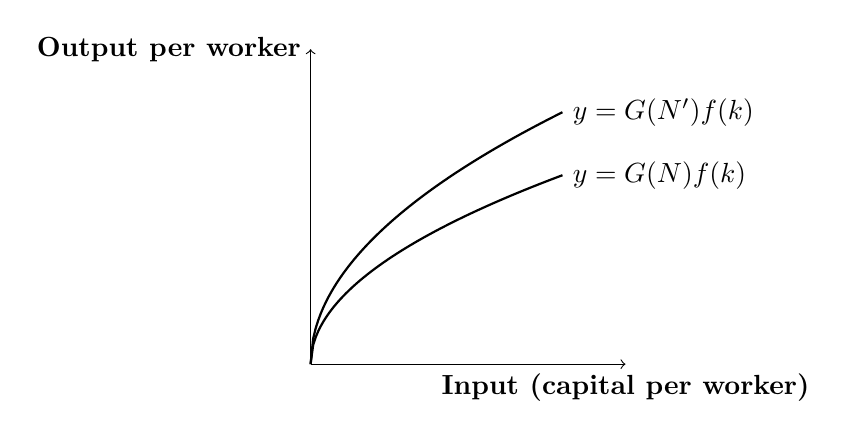
\begin{tikzpicture}[scale=0.8]
    % Axes
    \draw[->] (0,0) -- (5,0) node[below] {\textbf{Input (capital per worker)}} coordinate(x axis);
    \draw[->] (0,0) -- (0,5) node[left] {\textbf{Output per worker}} coordinate(y axis);
    
    % Curves
    \draw[thick, domain=0:4, samples=100] plot (\x, {1.5*sqrt(\x)}) node[right] {\( y = G(N)f(k) \)};
    \draw[thick, domain=0:4, samples=100] plot (\x, {2*sqrt(\x)}) node[right] {\( y = G(N')f(k) \)};
\end{tikzpicture}

\end{document}